%======================================================================
\chapter{Physics}
%======================================================================

\section{Refraction in a plasma}
In an unmagnetised plasma the dielectric permittivity and the refractive index at
angular frequency $\omega=2\pi f$ are
\begin{equation}
  \varepsilon = \mu^2 = 1-\frac{\omega_p^2}{\omega^2} = 1-\frac{n_e}{n_\text{cr}},
  \qquad
  n_\text{cr}=\frac{\pi m_e f^2}{e^2/(4\pi\varepsilon_0)}
  \approx 1.24\times10^{14}\left(\frac{f}{100\,\text{MHz}}\right)^2\ \text{m}^{-3}.
  \label{eq:ncr}
\end{equation}
The expression for $n_\text{cr}$ is \code{NElectronSiCr} in \code{ModRadioWaveImage.f90}
and \code{critical\_density()} in \code{constants.py}. Waves cannot propagate where
$n_e>n_\text{cr}$. The \emph{critical surface} $n_e=n_\text{cr}$ acts as a mirror.

\section{Ray equation}
From Fermat's principle $\delta\!\int\mu\,ds=0$, with the arc length $s$ as parameter
and $\vect v=d\vect r/ds$ ($|\vect v|=1$) (Benkevitch et al.\ 2010; Moschou et al.\
2018, Eq.~7):
\begin{equation}
  \frac{d\vect r}{ds}=\vect v,\qquad
  \frac{d\vect v}{ds}=\vect v\times\left(\frac{\nabla\mu}{\mu}\times\vect v\right)
  =\frac{\nabla\mu}{\mu}-\vect v\left(\vect v\cdot\frac{\nabla\mu}{\mu}\right),
  \qquad \frac{\nabla\mu}{\mu}=\frac{\nabla\varepsilon}{2\varepsilon},\quad
  \nabla\varepsilon=-\frac{\nabla n_e}{n_\text{cr}}.
  \label{eq:ray}
\end{equation}
The direction $\vect v$ only rotates, by the vector
$\vect\Omega=(\nabla\mu/\mu)\times\vect v$. This is the same as a charged particle
gyrating in a magnetic field, which is why the Boris scheme for particle pushers can be
used. The curvature of the ray is $\kappa=|\vect\Omega|=|\nabla_\perp\varepsilon|/(2\varepsilon)$.

\section{Emission and absorption}
\paragraph{Bremsstrahlung} (\code{ModUserAwsom.f90}; Moschou et al.\ 2018, Eqs.~15--16;
Rayleigh--Jeans limit $h\nu\ll k_BT_e$):
\begin{align}
  B_\nu &= \frac{2\nu^2k_BT_e}{c^2}, \\
  \kappa_\nu &= \frac43\sqrt{\frac{2\pi}{3}}\;
     \frac{\left[e^2/(4\pi\varepsilon_0)\right]^3}{c\,(k_BT_e m_e)^{3/2}}\;
     \frac{n_e^2}{\nu^2}\;\langle g_\text{ff}\rangle ,\qquad \langle g_\text{ff}\rangle=10 .
\end{align}
With \code{gaunt="dulk"} the Coulomb-logarithm form of Dulk (1985) is used instead:
$\kappa=9.78\times10^{-3}\,n_e^2\nu^{-2}T_e^{-3/2}\,G$ (cgs), where
$G=18.2+\ln T^{3/2}-\ln\nu$ for $T<2\times10^5$\,K and $G=24.5+\ln T-\ln\nu$ above.

\paragraph{Simplistic} (Benkevitch et al.\ 2010): $B=1$ and
$\kappa\,\rsun=(n_e/n_\text{cr})^2(0.5-n_e/n_\text{cr})^2$, giving a dimensionless
intensity.

\section{Intensity, brightness temperature and flux}
Optically thin, as in BATS-R-US (\code{transfer="thin"}):
\begin{equation}
  I_\nu=\sum_\text{segments}\kappa_\nu B_\nu\,\Delta\ell .
\end{equation}
Full formal solution of $dI/ds=\kappa(B-I)$, integrated from the observer into the
medium (\code{transfer="full"}):
\begin{equation}
  I_\nu=\sum_\text{segments}B_\nu\,e^{-\tau}\left(1-e^{-\Delta\tau}\right),\qquad
  \Delta\tau=\kappa_\nu\Delta\ell,\quad \tau\leftarrow\tau+\Delta\tau .
\end{equation}
Here $\tau$ is the optical depth accumulated between the observer and the start of the
segment. The brightness temperature and the flux density at distance $D$ are
\begin{equation}
  T_b=\frac{c^2 I_\nu}{2k_B\nu^2},\qquad
  F_\nu=\sum_\text{pixels}I_\nu\,\Delta\Omega,\quad \Delta\Omega=\frac{\Delta X\,\Delta Y}{D^2}.
\end{equation}

%======================================================================
\chapter{Numerical algorithm}
%======================================================================

\section{Image set-up}
This follows \code{write\_plot\_radiowave}. The pixel centres are
$X_i=-X_\text{size}/2+(i-\tfrac12)\Delta X$ and $Y_j=-Y_\text{size}/2+(j-\tfrac12)\Delta Y$.
Their positions in space are $\vect P_{ij}=X_i\hat\tau+Y_j\hat\xi$, and the ray
directions are $\vect v_0=(\vect P_{ij}-\vect O)/|\vect P_{ij}-\vect O|$.

In BATS-R-US the ray starts where it meets the integration sphere,
$r_\text{int}=\lceil\max(\sqrt{(X_\text{size}/2)^2+(Y_\text{size}/2)^2}+1,\,5)\rceil$.
\code{radiosynth} starts it at the later of two points: that entry point and the point
where the ray enters the model domain. This matters when the model box is smaller than
the integration sphere. The vacuum segment in front contributes nothing.

\section{One integration step}
All active rays advance together. One step from $(\vect r_0,\vect v_0)$ with step
$\Delta s$ consists of the following (Fig.~\ref{fig:flow}).

\begin{enumerate}[itemsep=3pt]
\item \textbf{Predictor:} $\vect r_{1/2}=\vect r_0+\vect v_0\,\Delta s/2$. Sample
      $n_e$, $\nabla n_e$, $T_e$ and the local cell size there.
\item \textbf{Termination tests:} the ray stops if $r_{1/2}<r_\text{body}$ (the
      remaining straight piece to the surface is still integrated), if it has left the
      domain or the integration sphere, or if $n_e\ge n_\text{cr}$.
\item \textbf{Permittivity:} $\varepsilon_{1/2}=1-n_e/n_\text{cr}$ and
      $\nabla\varepsilon=-\nabla n_e/n_\text{cr}$. Extrapolate back to the start of the
      step: $\varepsilon_0=\varepsilon_{1/2}-(\nabla\varepsilon\cdot\vect v_0)\,\Delta s/2$.
      If $\varepsilon_0\le0$ the ray has crossed the critical surface.
\item \textbf{Recovery} (default mode only): if the ray is over-dense or
      $\varepsilon_0\le0$, retry with $\Delta s/4$. Once $\Delta s<4\,\Delta s_\text{min}$,
      reflect it specularly:
      $\vect v\leftarrow\vect v-2(\vect v\cdot\hat g)\hat g$ with
      $\hat g=\nabla\varepsilon/|\nabla\varepsilon|$.
\item \textbf{Precision control} (\code{check\_step}, only for rays not yet marked steep):
  \begin{itemize}[itemsep=1pt]
   \item curvature: if $\left(\kappa\,\Delta s/2\right)^2=\left(\frac{\Delta s}{4\varepsilon_0}\right)^2
         \left(|\nabla\varepsilon|^2-(\nabla\varepsilon\cdot\vect v_0)^2\right)\ge\text{Tol}^2$,
         set $\Delta s\leftarrow0.99\,\Delta s\,\text{Tol}/(2\kappa\Delta s/2)$ and redo
         the step;
   \item correctness (Benkevitch Eq.~33): if
         $3(\nabla\varepsilon\cdot\vect v_0)\,\Delta s/2\le-\varepsilon_0$, a linear
         prediction says the ray will reach $\varepsilon=0$ within about $1.5\,\Delta s$.
         Mark the ray \emph{steep}, store the distance to the critical surface
         $d_\text{cr}=\varepsilon_0/|\nabla\varepsilon|$, set
         $\Delta s\leftarrow\max(\tfrac12\text{Tol}\,d_\text{cr},\ \text{StepMin})$ and redo
         the step.
  \end{itemize}
\item \textbf{Advance} (\code{advance\_ray}):
  \begin{itemize}[itemsep=1pt]
  \item no refraction: $\vect r_1=\vect r_{1/2}+\vect v_0\Delta s/2$;
  \item parabolic switch, if $3(\nabla\varepsilon\cdot\vect v_0)\Delta s/2\le-\varepsilon_0$
        (see \S\ref{sec:parab});
  \item otherwise a Boris step (\S\ref{sec:boris}).
  \end{itemize}
  The segment adds $\kappa B\,\Delta\ell$ (thin) or $B e^{-\tau}(1-e^{-\Delta\tau})$
  (full) to the pixel, with $\kappa$, $B$ evaluated at $\vect r_{1/2}$. If the step
  ends inside $r_\text{body}$ it is clipped at the surface.
\item \textbf{Exit test:} stop the ray if $\vect r_1$ is outside the domain or the
      integration sphere.
\item \textbf{Step regrowth} (\code{get\_new\_step\_size}): for gentle rays, and for
      steep rays that have moved away from the critical surface
      ($\varepsilon_0>d_\text{cr}|\nabla\varepsilon|$),
      \[\Delta s\leftarrow\max\!\left(2-\frac{\Delta s}{\Delta s_\text{new}},1\right)
        \min(\Delta s_\text{new},\Delta s),\qquad \Delta s_\text{new}=\text{step\_factor}\times\text{cell size}.\]
      This grows small steps geometrically and saturates smoothly at
      $\Delta s_\text{new}$.
\end{enumerate}

\begin{figure}[p]
\centering
\begin{tikzpicture}[node distance=7mm and 8mm, >=Stealth, font=\small,
  box/.style={draw,rounded corners=2pt,fill=notebg,align=center,minimum width=4.6cm,inner sep=4pt},
  dec/.style={draw,diamond,aspect=2.6,fill=warnbg,align=center,inner sep=1pt},
  term/.style={draw,rounded corners=6pt,fill=gray!15,align=center,inner sep=4pt}]
\node[box] (pred) {predictor $\vect r_{1/2}=\vect r_0+\vect v_0\Delta s/2$\\ sample $n_e,\nabla n_e,T_e$, cell};
\node[dec, below=of pred] (stop) {outside / body /\\ $n_e\ge n_\text{cr}$?};
\node[term, right=12mm of stop] (end) {stop ray\\(body: integrate\\to surface)};
\node[box, below=of stop] (eps) {$\varepsilon_{1/2}$, $\nabla\varepsilon$,\\ $\varepsilon_0=\varepsilon_{1/2}-\nabla\varepsilon\cdot\vect v_0\,\Delta s/2$};
\node[dec, below=of eps] (neg) {$\varepsilon_0\le0$ or\\over-dense?};
\node[box, left=10mm of neg, minimum width=3.2cm] (rec) {recovery:\\$\Delta s/4$ or Snell\\reflection};
\node[dec, below=of neg] (curv) {curvature\\$\kappa\Delta s/2\ge$ Tol?};
\node[box, left=10mm of curv, minimum width=3.2cm] (shr) {shrink $\Delta s$,\\redo step};
\node[dec, below=of curv] (steep) {$3\nabla\varepsilon\cdot\vect v\,\Delta s/2$\\$\le-\varepsilon_0$ ?};
\node[box, left=10mm of steep, minimum width=3.2cm] (mk) {mark steep,\\$\Delta s=\max(\frac{\text{Tol}}{2}d_\text{cr},$\\ StepMin), redo};
\node[box, below=9mm of steep] (adv) {advance: straight / parabola / Boris\\add emission of the segment};
\node[box, below=of adv] (grow) {exit test; regrow $\Delta s$ towards cell size};
\draw[->] (pred) -- (stop);
\draw[->] (stop) -- node[above]{yes} (end);
\draw[->] (stop) -- node[right]{no} (eps);
\draw[->] (eps) -- (neg);
\draw[->] (neg) -- node[above]{yes} (rec);
\draw[->] (neg) -- node[right]{no} (curv);
\draw[->] (curv) -- node[above]{yes} (shr);
\draw[->] (curv) -- node[right]{no} (steep);
\draw[->] (steep) -- node[above]{yes} (mk);
\draw[->] (steep) -- node[right]{no / already steep} (adv);
\draw[->] (adv) -- (grow);
% loop back on the right (next step)
\coordinate (R) at ($(end.east)+(0.6,0)$);
\draw[->] (grow.east) -- (grow.east -| R) -- (pred.east -| R) -- node[above,pos=0.5]{next step} (pred.east);
% loop back on the left (redo the same step)
\coordinate (Lft) at ($(mk.west)+(-0.6,0)$);
\draw (rec.west) -- (rec.west -| Lft);
\draw (shr.west) -- (shr.west -| Lft);
\draw (mk.west) -- (mk.west -| Lft) -- (pred.west -| Lft);
\draw[->] (pred.west -| Lft) -- node[above,pos=0.5]{redo} (pred.west);
\node[gray,align=left,font=\scriptsize,anchor=west] at ($(curv.east)+(0.3,0)$) {steep rays skip\\the two precision\\tests};
\end{tikzpicture}
\caption{Flow of one integration step for one ray (\code{trace\_rays}). All active rays
pass through it together, as boolean masks over arrays.}\label{fig:flow}
\end{figure}

\section{Boris (CYLRAD) step}\label{sec:boris}
With $\vect a=\dfrac{\nabla\varepsilon}{2\varepsilon_{1/2}}\dfrac{\Delta s}{2}$
($=\nabla\mu/\mu\cdot\Delta s/2$; code variable \code{rel}), Benkevitch et al.\ (2010,
Eq.~24) write
\begin{align}
  \vect\Omega_0 &= \vect a\times\vect v_0, &
  \vect v' &= \vect v_0+\vect v_0\times\vect\Omega_0, \nonumber\\
  \vect\Omega_{1/2} &= \vect a\times\vect v', &
  \vect v'' &= \vect v_0+\vect v_0\times\vect\Omega_{1/2}, \nonumber\\
  \vect v_1 &= \vect v_0+\frac{2}{1+\Omega_{1/2}^2}\,\vect v''\times\vect\Omega_{1/2}, &
  \vect r_1 &= \vect r_{1/2}+\vect v_1\frac{\Delta s}{2}.
\end{align}
The rotation keeps $|\vect v|=1$ exactly, and the scheme is second-order accurate.

\section{Parabolic switch at the critical surface}\label{sec:parab}
If $\nabla\varepsilon$ is constant over the step, the ray is a parabola. Let $\alpha$ be
the angle between $\vect v_0$ and $-\nabla\varepsilon$, and $L=1/|\nabla\varepsilon|$.
Then
\begin{align*}
  L\cos\alpha &= -\frac{\nabla\varepsilon\cdot\vect v_0}{|\nabla\varepsilon|^2}, &
  \vect v_\parallel &= -L\cos\alpha\,\nabla\varepsilon\quad(\text{component of }\vect v_0\text{ along }\nabla\varepsilon),\\
  \vect v_1 &= \vect v_0-2\vect v_\parallel, &
  \Delta\vect r_\perp &= 4\,(\vect v_0-\vect v_\parallel)\,L\cos\alpha\,\varepsilon_0,\\
  \vect r_1 &= \vect r_0+\Delta\vect r_\perp, &
  \Delta\vect r_\parallel &= \varepsilon_0(L\cos\alpha)^2\,\nabla\varepsilon,\qquad
  \Delta\ell=\sqrt{|2\Delta\vect r_\parallel|^2+|\Delta\vect r_\perp|^2}.
\end{align*}
The ray jumps to the symmetric point on the other branch of the parabola. Its normal
velocity component is reversed, and the emission of the parabolic arc is counted over the
length $\Delta\ell$.

\section{Distant observers (stars)}
For a star at distance $D$ (\code{distance\_pc}) the rays are parallel to $-\hat n$. The
ray of pixel $(i,j)$ passes through $\vect P_{ij}=X_i\hat\tau+Y_j\hat\xi$ and starts
outside the model at $\vect P_{ij}+R_\text{far}\hat n$. The pixel solid angle is
$\Delta X\Delta Y/D^2$, and the flux $F_\nu=\sum I_\nu\,\Delta X\Delta Y/D^2$ with all lengths in
the same unit. Path lengths are converted to metres with the grid's \code{length\_unit}
($R_\odot$ or $R_\ast$).

\section{Relation to BATS-R-US}
The ray tracer is written following the radio-wave imaging module of BATS-R-US
(\code{ModRadioWaveImage.f90}, with the image set-up of \code{ModWritePlotRadioWave.f90}
and the emission coefficients of \code{ModUserAwsom.f90}). The defaults of the
numerical parameters (\code{tolerance}, \code{step\_min}) are those of BATS-R-US, and
\code{strict\_batsrus=True} reproduces its step logic exactly
(Section~\ref{sec:strict}). In \code{radiosynth} the step is organised in small
subroutines (predictor, terminations, permittivity, step control, advance, emission,
step regrowth) that act on all rays at once; they are described line by line in the
Code Reference.

%======================================================================
\chapter{Gyroresonance emission and polarised transfer}\label{chap:grtheory}
%======================================================================

This chapter describes the physics of the \code{gyroresonance} folder and of the
magnetised free--free coefficients in \code{bremsstrahlung/magnetized.py}.

\section{Magneto-ionic modes}
With $X=(\nu_p/\nu)^2=n_e/n_\text{cr}$, $Y=\nu_B/\nu$, $\nu_B=eB/(2\pi m_e)=2.7992$\,MHz\,$B$[G],
and $\theta$ the angle between $\vect B$ and the wave vector $\vect k$ (pointing to the
observer), a cold magnetised plasma supports two modes, the extraordinary (x) mode whose
electric vector rotates with the electrons and the ordinary (o) mode. Their refractive
indices are given by the Appleton--Hartree formula
\begin{equation}
  n_{o,x}^2 = 1-\frac{X(1-X)}{(1-X)-\tfrac12Y^2\sin^2\theta\pm\sqrt{\tfrac14Y^4\sin^4\theta+(1-X)^2Y^2\cos^2\theta}},
\end{equation}
with cutoffs at $X=1$ (o) and $X=1-Y$ (x). In the frame with $\vect B\parallel\hat z$ and
$\vect k$ in the $x$--$z$ plane, the transverse polarisation vector of mode $\sigma$ is
$\vect e_\sigma=(T_\sigma\cos\theta,\,i,\,-T_\sigma\sin\theta)/\sqrt{1+T_\sigma^2}$
(longitudinal part neglected), with $T_oT_x=-1$ and
\begin{equation}
  |T_x| = \frac{2(1-X)|\cos\theta|}{Y\sin^2\theta+\sqrt{Y^2\sin^4\theta+4(1-X)^2\cos^2\theta}} .
\end{equation}
Along $\vect B$ the modes are circular ($|T|=1$); across $\vect B$ the x-mode is linear with
$\vect E\perp\vect B$ ($T_x=0$) and the o-mode linear with $\vect E\parallel\vect B$.
For $\vect B\cdot\vect k>0$ the x-mode is right-hand circularly polarised in the IAU/IEEE
convention, i.e.\ contributes $V>0$.

\section{Gyroresonance opacity of a harmonic layer}
An electron of perpendicular velocity $\beta_\perp c$ radiates at the harmonics
$s\nu_B$ (Doppler-shifted by its parallel motion). For a wave of polarisation
$\vect e_\sigma$ the coupling to the $s$-th harmonic contains the Bessel functions
$J_{s\pm1}(x)$ and $J_s(x)$ of argument $x=s\beta_\perp\sin\theta$ (Schott's formula). In
the corona $\beta_T^2=k_BT_e/(m_ec^2)\approx3\times10^{-4}$, so $x\ll1$ and
$J_{s-1}(x)\simeq(x/2)^{s-1}/(s-1)!$ dominates for the co-rotating component. Averaging
over a Maxwellian, with $\langle\beta_\perp^{2n}\rangle=n!\,(2\beta_T^2)^n$, gives
\begin{equation}
  s\,\big\langle J_{s-1}^2(s\beta_\perp\sin\theta)\big\rangle
   = \frac{s^2}{s!}\left(\frac{s^2\beta_T^2\sin^2\theta}{2}\right)^{s-1}\big[1+O(s^2\beta_T^2)\big].
\end{equation}
The absorption coefficient is a narrow line in frequency, of Doppler width
$\sim\nu\beta_T|\cos\theta|$ around $s\nu_B$. Along a ray $\nu_B$ varies, so the line
is crossed in a layer of thickness $\sim L_B\beta_T$, where $L_B=|B/(dB/d\ell)|$. The
integral of the line profile across the layer is independent of the profile and gives
the optical depth of the layer (Zheleznyakov 1970; White \& Kundu 1997; Fleishman \&
Kuznetsov 2014)
\begin{equation}
  \tau_s^\sigma=\frac{\pi e^2}{m_ec}\,\frac{n_eL_B}{\nu}\;\frac{s^2}{s!}
   \left(\frac{s^2\beta_T^2\sin^2\theta}{2}\right)^{s-1}F_\sigma(\theta),\qquad
  F_\sigma=\frac{(1+T_\sigma\cos\theta)^2}{1+T_\sigma^2},
  \label{eq:grtau}
\end{equation}
in cgs ($\pi e^2/m_ec=0.02654$\,cm$^2$\,s$^{-1}$; in SI $e^2\to e^2/4\pi\varepsilon_0$),
with $T_\sigma$ evaluated at $Y=1/s$ and signed so that $T_x\cos\theta>0$:
$F_x=(1+|T_x||\cos\theta|)^2/(1+T_x^2)$, $F_o=(|T_x|-|\cos\theta|)^2/(1+T_x^2)$.
Along $\vect B$, $F_x=2$ and $F_o=0$; across $\vect B$, $F_x=1$ and $F_o=0$ at this order.
The refractive index $n_\sigma^{2s-3}$ of the full expression is set to 1 ($X\ll1$).

Orders of magnitude for $n_e=10^9$\,cm$^{-3}$, $L_B=10^9$\,cm, $T_e=2$\,MK at 5\,GHz,
$\theta=60^\circ$: $\tau_2^x\approx7\times10^{3}$, $\tau_3^x\approx12$,
$\tau_4^x\approx0.03$, with $\tau^o$ smaller by a factor 20--50. The $s=2$ and $s=3$
layers are therefore usually thick in the x-mode, $s=2$ often also in the o-mode, and
$s\ge4$ thin. At $s=1$ ($Y=1$) the x-mode is cut off for any $X>0$, so only the o-mode
reaches that layer.

\paragraph{Kirchhoff's law} holds for each mode separately: a thermal layer emits the
source function $S_\sigma=\nu^2k_BT_e/c^2$ (half the Rayleigh--Jeans intensity), so a thick
layer has $T_b=T_e$ in that mode.

\section{Magnetised free--free absorption}
For $Y<1$ and away from quasi-transverse propagation (Dulk 1985; Zheleznyakov 1970)
\begin{equation}
  \kappa_\sigma=\frac{\kappa_\text{ff}}{(1+\sigma Y|\cos\theta|)^2},\qquad
  \sigma=+1\ (\text{o}),\ -1\ (\text{x}),
\end{equation}
with $\kappa_\text{ff}$ the unmagnetised coefficient. For an optically thin source this
gives $V/I=2q/(1+q^2)\approx2Y|\cos\theta|$ with $q=Y|\cos\theta|$, and $V\to0$ for a thick
isothermal source.

\section{Transfer along straight rays}
Each line of sight is sampled at equal steps (\code{common/straight.py}). For step $k$
between nodes $k$ and $k+1$ the code computes, for both modes,
\begin{itemize}[itemsep=1pt]
\item the free--free optical depth $\kappa_\sigma\Delta\ell$ at the mid-point;
\item for every harmonic whose layer field $|B|=\nu/(s\nu_B/\text{G})$ lies between the
  field strengths at the two nodes, the layer optical depth \eqref{eq:grtau}, with
  $n_e$, $T_e$, $\theta$ interpolated to the crossing and
  $L_B=|B|\,\Delta\ell/|B_{k+1}-B_k|$;
\item the source function of the step, the $\tau$-weighted mean of $\nu^2k_BT/c^2$ over
  its free--free part and its layers.
\end{itemize}
Then
\begin{equation}
  I_p=\sum_k S_k\left(1-e^{-\Delta\tau_k}\right)e^{-\sum_{j<k}\Delta\tau_j},
\end{equation}
summed from the observer inwards, for the two polarisations $p$; a polarisation stops at
its cutoff. The layer itself is much thinner than a step ($L_B\beta_T\ll\Delta\ell$), so
treating it as a discontinuity is exact as long as $L_B$ is resolved.

\paragraph{Mode coupling.} Where $\vect B\cdot\vect k$ changes sign along a ray (a
quasi-transverse region), the modes either keep their identity and the sense of
polarisation flips (strong coupling, low frequencies, strong fields) or keep their sense
of polarisation and exchange identity (weak coupling, usual at microwaves; Cohen 1960).
With \code{coupling="weak"} the transfer is done for right- and left-hand circular
polarisation: $R$ uses the x-mode coefficients where $\vect B\cdot\vect k>0$ and the
o-mode ones elsewhere, $L$ the opposite; $I=R+L$, $V=R-L$. With \code{coupling="strong"}
the transfer is done for the x- and o-modes and $V=\pm(I_x-I_o)$ with the sign of
$\vect B\cdot\vect k$ at the observer's end of the ray.

\paragraph{Diagnostics.} The contribution of each step to $I$ is split between its
free--free part and its layers. The harmonic whose layers contribute most is reported as
\code{dominant\_s}, the contribution-weighted radius as \code{radius}, and the layer share
as \code{gr\_fraction}.

%======================================================================
\chapter{Gyrosynchrotron emission through the fast GS codes}\label{chap:gstheory}
%======================================================================

For a distribution of fast electrons $f(E,\mu)$ the emissivity and absorption coefficient
of each magneto-ionic mode are sums over gyroharmonics of integrals over energy and pitch
angle involving the Bessel functions $J_s$ and $J'_s$ (e.g.\ Melrose 1968; Ramaty 1969).
The fast codes (Fleishman \& Kuznetsov 2010) evaluate these exactly below a switch
frequency $f_C$ (in units of the local gyrofrequency; with exact Bessel functions below
$f_{WH}$ and the Wild \& Hill (1971) approximation above) and with a continuous
(harmonic-averaged) formula above it, with a renormalisation that makes the spectrum
continuous. The 2021 version adds numerically defined distributions, more analytical
distributions, the free--free contribution of electron--ion and electron--neutral
collisions with selectable abundances, and the radiative transfer along a line of sight
with weak, strong or exact mode coupling.

\paragraph{Interface.} For each pixel radiosynth passes the voxels of its straight line
of sight in the order the codes expect (from the far end to the observer), each with
\begin{equation*}
 \Delta z\,[\text{cm}],\ T_e,\ n_e\,[\text{cm}^{-3}],\ |\vect B|,\
 \theta=\arccos\frac{\vect B\cdot\hat{\vect n}_\text{obs}}{|\vect B|},\ 
 \text{and } n_b, \delta, E_\text{min}, E_\text{max}, \ldots
\end{equation*}
(the proton density is set equal to $n_e$, which tells the codes that $n_e$ is the electron
density also below $10^5$\,K). The codes return the flux densities of the left and right
circular polarisations, in sfu, that a source of area $S$ would produce at 1\,AU. With
$S$ = the pixel area, the intensity is
\begin{equation}
  I_{L,R}=F_{L,R}\,\frac{10^{-22}\,\text{W m}^{-2}\text{Hz}^{-1}\,(1\,\text{AU})^2}{S},
\end{equation}
independent of the actual observer distance; $V=I_R-I_L$. These conventions are checked
in \code{tests/test\_gyrosynchrotron.py}: the image of a uniform slab equals a direct call
of the library on the same voxels; an optically thick thermal slab gives $T_b=n^2T_e$
exactly; for $\vect B\cdot\hat{\vect n}_\text{obs}>0$ the thin emission is right-hand
polarised and reversing $\vect B$ reverses $V$; and the thin free--free polarisation
equals $2q/(1+q^2)$ as in radiosynth.

%======================================================================
\chapter{Combining the mechanisms in one transfer}\label{chap:cbtheory}
%======================================================================

For each circular polarisation $p$ and each step $k$ of a straight line of sight, the
contributions $i$ (free--free, the harmonic layers in the step, and the gyrosynchrotron
emission of the fast electrons) have optical depths $\Delta\tau_{i}$ and source functions
$S_{i}$. For a homogeneous step with total absorption $\sum_i\kappa_i$ and emissivity
$\sum_i j_i$ the formal solution has
\begin{equation}
  \Delta\tau_k=\sum_i\Delta\tau_i,\qquad
  S_k=\frac{\sum_i j_i}{\sum_i\kappa_i}=\frac{\sum_i\Delta\tau_i S_i}{\sum_i\Delta\tau_i},
\end{equation}
and $I_p=\sum_k S_k(1-e^{-\Delta\tau_k})e^{-\sum_{j<k}\Delta\tau_j}$ as before. Thermal
contributions have $S_i=\nu^2k_BT_e/c^2$; for the gyrosynchrotron part
$S=E/(1-e^{-\tau})$ with $\tau$ and $E$ from the one-voxel calls of the fast GS codes
(for $I_\text{in}=0$: $I_\text{out}=E$; for a known $I_\text{in}$:
$I_\text{out}=I_\text{in}e^{-\tau}+E$). The share of each process in a pixel is the sum
over steps of $S_k(1-e^{-\Delta\tau_k})e^{-\tau_{<k}}\times\Delta\tau_iS_i/\sum_i\Delta\tau_iS_i$.

Checks (\code{tests/test\_combined.py}): without fast electrons the result is identical to
the gyroresonance image; with only the gyrosynchrotron part it reproduces the codes' own
line-of-sight transfer to $10^{-15}$; in the optically thin limit it equals the sum of
the separate contributions; a thick layer in front of a gyrosynchrotron source yields
$T_b=T_e$ of the layer.

%======================================================================
\chapter{Validation}\label{chap:validation}
%======================================================================

The test scripts in \code{tests/} compare \code{radiosynth} with analytic solutions,
with an independent ODE integration, and against itself across input formats. A
spherically symmetric Newkirk corona ($n_e=4.2\times10^{4}\cdot10^{4.32/r}$\,cm$^{-3}$,
$T_e=1.5$\,MK) on a 0.025\,\rsun{} grid is used unless stated otherwise.

\begin{table}[h]\centering\small
\begin{tabularx}{\textwidth}{@{}X l@{}}
\toprule
Test & Result \\
\midrule
Bouguer invariant $\mu r\sin\psi$ conserved along rays (80\,MHz) & 1.2\% max.\ deviation \\
Turning radius vs.\ analytic $\mu(r_0)r_0=b$ & $4\times10^{-4}\,\rsun$ \\
Exit direction vs.\ \code{scipy solve\_ivp} of Eq.~\eqref{eq:ray} (150\,MHz) & $\le0.3^\circ$ (0.03$^\circ$ on exact field) \\
Straight-ray intensity vs.\ quadrature (1, 17\,GHz) & $\le0.9\%$ \\
Full transfer: $T_b\le T_e$ & yes \\
Flux vs.\ step size (step\_factor 1 $\to$ 0.25, 150\,MHz) & $3\times10^{-4}$ \\
Tecplot ASCII / IDL real4 / IDL ascii readers & exact (float32) \\
Scattered points resampled & $3\times10^{-3}$ \\
PLUTO 3D spherical \code{.dbl} vs.\ Cartesian reference (80--1000\,MHz) & flux 1--3.5\%, corr.\ 0.9999 \\
PLUTO 2.5D axisymmetric \code{.flt} & flux 1.4\% \\
PLUTO VTK vs.\ \code{.dbl} & identical \\
pyPLUTO reader vs.\ built-in reader & identical (float32) \\
Ephemeris vs.\ Meeus ex.\ 29.a ($P$, $B_0$, $L_0$) & $\le0.02^\circ$ \\
Longitude-offset fit (known $+17^\circ$) & $+16.8^\circ$ \\
Stellar wind: $\tau$ per pixel vs.\ analytic & $0.08\%$ \\
Stellar wind: flux vs.\ exact; analytic $S_\nu$ vs.\ quadrature & $0.02\%$; $10^{-7}$ \\
Coordinates in $R_\odot$ vs.\ $R_\ast$ & identical \\
\midrule
\multicolumn{2}{@{}l}{\emph{Gyroresonance (\code{tests/test\_gyroresonance.py})}}\\
Layer $\tau_s$ vs.\ Maxwellian average of exact $J_{s-1}^2$ ($s=2$--6) & $\le0.8\%$ (= $O(s^2\beta_T^2)$) \\
Single $s=3$ layer in a linear field: $I=S(1-e^{-\tau})$ per mode & $10^{-6}$ \\
Thick layers: $T_b(R)=T_b(L)=T_e$ & $2\times10^{-11}$ \\
$V$ sign over the positive spot; $\vect B\to-\vect B$ gives $V\to-V$ & exact \\
Straight-ray free--free vs.\ refractive tracer without refraction & $5\times10^{-4}$ \\
Thin magnetised free--free: $V/I=2q/(1+q^2)$ & $3\times10^{-4}$ \\
SphericalGrid $(B_r,B_\theta,B_\phi)$ vs.\ Cartesian image ($I$; $V$) & 0.8\%; 1.8\% \\
PLUTO \code{bx1..3} code units $\to$ gauss & $10^{-11}$ \\
\code{compare\_refraction} vs.\ separate runs; 17\,GHz refracted/straight flux & identical; $1-2\times10^{-4}$ \\
\midrule
\multicolumn{2}{@{}l}{\emph{Combined image (\code{tests/test\_combined.py})}}\\
No fast electrons vs.\ \code{make\_gr\_image} & identical \\
Gyrosynchrotron alone (per-voxel coefficients) vs.\ library transfer & $10^{-15}$ \\
Per-voxel $\tau$: probe intensity 1 vs.\ $10^4$\,sfu & $3\times10^{-12}$ \\
Thin: combined vs.\ sum of contributions; thick: combined/sum & $8\times10^{-6}$; 0.98 \\
Thick layer in front of a gyrosynchrotron source & $T_b=T_e$ \\
Fractions sum; $\vect B\to-\vect B$ & 1; $V\to-V$ ($10^{-15}$) \\
\code{ff\_refraction} (free--free only) vs.\ refracted \code{make\_radio\_image} & $\le1.1\times10^{-3}$ \\
\midrule
\multicolumn{2}{@{}l}{\emph{1D models (\code{tests/test\_symmetric.py})}}\\
Symmetric image (one row of rays) vs.\ full 2D image: flux; $T_b$ along a row & $2\times10^{-4}$; $3\times10^{-4}$ \\
1D profile grid vs.\ 3D Cartesian grid of the same corona & 0.02--2\% \\
Optically thick wind from a text table: profile flux vs.\ exact integral & $2\times10^{-4}$ \\
PLUTO 1D \code{.dbl} read as a symmetric model & $4\times10^{-4}$ \\
\midrule
\multicolumn{2}{@{}l}{\emph{Gyrosynchrotron (\code{tests/test\_gyrosynchrotron.py})}}\\
Image of a uniform slab vs.\ direct library call & $3\times10^{-7}$ \\
Thick thermal slab: $T_b=n^2T_e$ (sfu $\to$ intensity conversion) & $<10^{-4}$ \\
Thin emissivity vs.\ Dulk \& Marsh (1982), $\delta=3$--5, $\nu/\nu_B=20$--50 & ratio 1.3--2.0 (approximate fits) \\
$V$ sign for $\vect B$ towards the observer; $\vect B\to-\vect B$ & as expected; exact \\
Thin free--free from the library vs.\ radiosynth: $I$; $V/I$ & $+15\%$ (Coulomb log.); $\le3\%$ \\
Array-defined vs.\ analytical power law & $3\times10^{-3}$ \\
$|\vect J|$ of an analytic field; $n_b$ rules; energy check & exact \\
\bottomrule
\end{tabularx}
\caption{Validation summary.}
\end{table}

\begin{figure}[h]
\centering
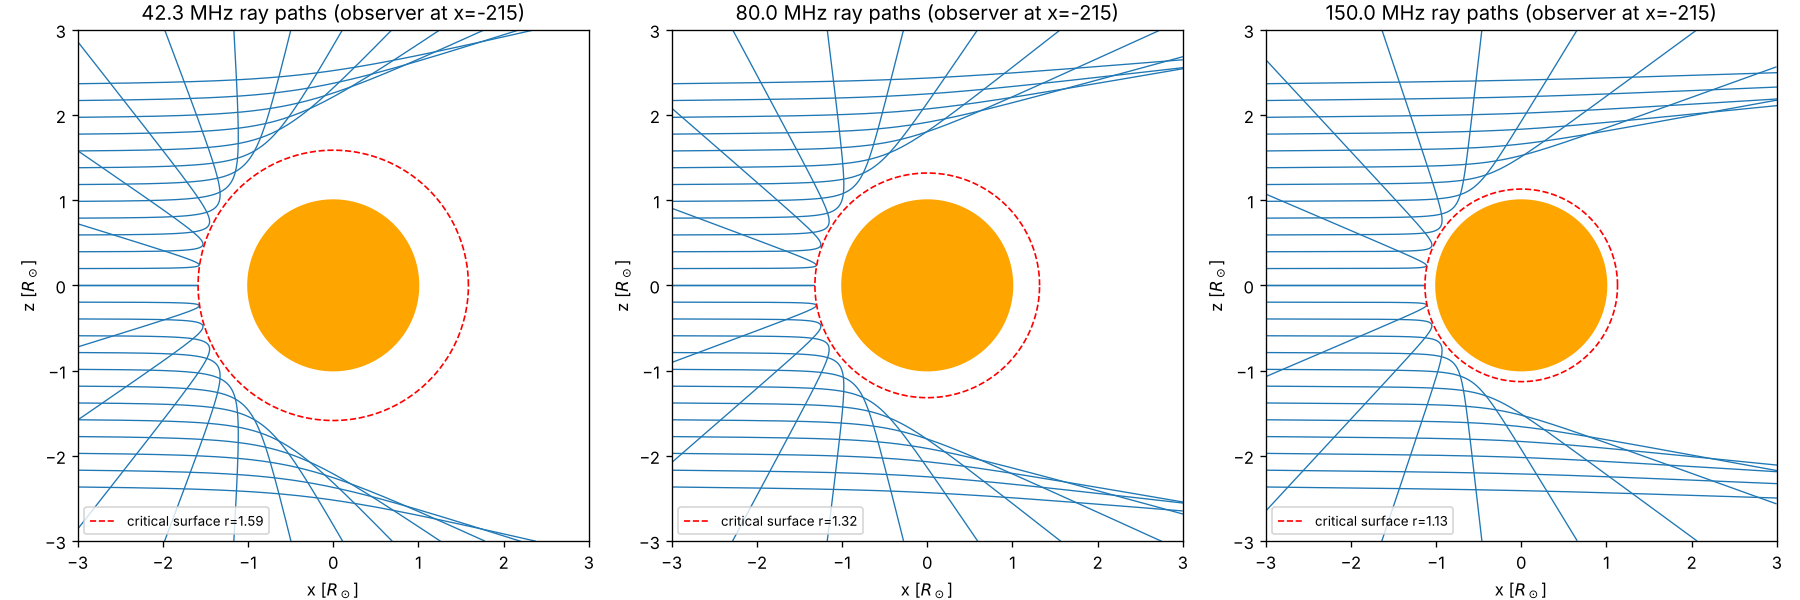
\includegraphics[width=\textwidth]{fig/ray_paths.png}
\caption{Ray paths in the Newkirk corona at 42.3, 80 and 150\,MHz, compare
Benkevitch et al.\ (2010), Figs.~7--9. Rays aimed at the disk turn back before
reaching the critical surface (red).}\label{fig:paths}
\end{figure}

\begin{figure}[h]
\centering
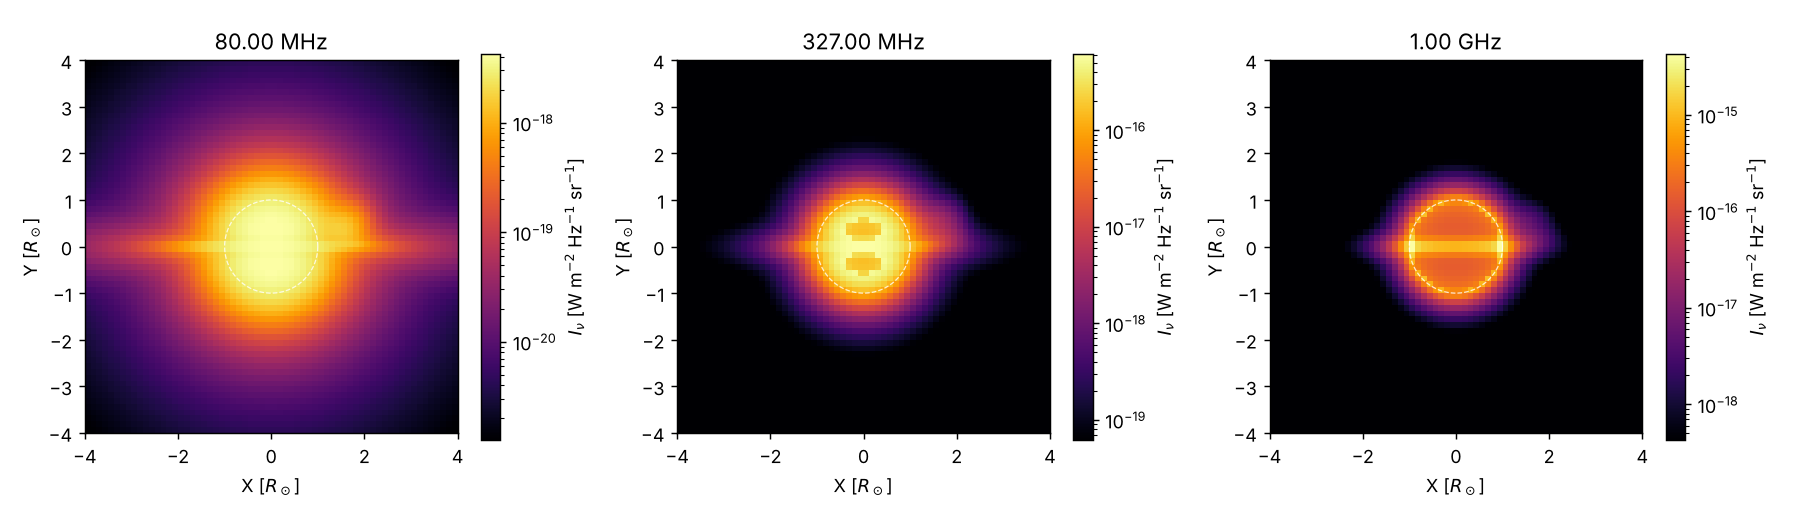
\includegraphics[width=\textwidth]{fig/pluto_sph_images.png}
\caption{Optically thin intensity computed from the synthetic PLUTO 3D spherical
output (\code{tests/test\_pluto.py}).}
\end{figure}
